\section{Active Features-based Model Selection (AFMS)}
\label{sec:testspeedup}
%
To speed up the classification time, our optimization technique AFMS
leverages properties of a soft-margin linear SVM model.  In this
model, the predicted label for a file $f$ is determined using the
score:
%
\vspace{-0.1in}
\begin{equation} 
\vspace{-0.1in}
\label{eq:linearsvmsum}
g(f) = w_0 + \sum_{j=1}^{F}{w_j*x_j}
\end{equation}
%
Here, $F$ is the number of features, $w_0$ is the intercept, $w_j$ 
is the $j^{th}$ feature weight in the model, and $x_j$ is the value of the $j^{th}$
feature of the file. The model predicts label $1$ if $g(f) \ge 0$,
and $0$ otherwise.  Given that our features have non-negative values,
without applying the model we can predict label $0$ when the following
conditions are met:
%
\begin{itemize}
  \renewcommand{\labelitemi}{$\bullet$}
  \item \textbf{condition 1}: The intercept is negative, i.e., $w_0 <
    0$, and
  \item \textbf{condition 2}: None of the weights of active (non-zero)
    features is positive.
\end{itemize}
%
Under these conditions, $g(f)$ is always negative, and hence the predicted label
is $0$.  Otherwise, we need to apply the model to obtain the
classification label, which could be 0 or 1.  The AFMS technique uses
this key intuition to save the cost of applying classification models.
Of course, its effectiveness depends on the number of times the
conditions are matched. Unsurprisingly, as our experiments show, this
happens quite often (refer Table~\ref{tab:SpeedupPotentialStats}):
%
\begin{itemize}
    \renewcommand{\labelitemi}{$\bullet$}
\item \textbf{condition 1}: Around $96\%$ of the metadata models have negative
  intercept (i.e., $w_0 < 0$).  This is because a typical user
  accesses only a small fraction of files.  Owing to this natural
  imbalance, the model favors $0$ as the prediction label, resulting
  in a negative intercept.
\item \textbf{condition 2}: Our data shows sparsity of features
  with an average of only $2.2\%$ of metadata features being active (i.e., $x_j > 0$) in the files.
  Also, the average ratio of the features with positive weights (i.e., $w_j > 0$) per model is only
  $6.4\%$, and each of these features on an average has a positive weight in less
  than $10\%$ of the models.  The combination of these three facts
  significantly lowers the probability of finding active features with positive
  weights.
\end{itemize}
\begin{table*}
{\fontsize{8pt}{1em}\selectfont
\begin{center}
%\begin{tabular}{|>{\centering}p{0.065\linewidth}|>{\centering}p{0.2\linewidth}|>{\centering}p{0.25\linewidth}|>{\centering}p{0.2\linewidth}|>{\centering}p{0.23\linewidth}|}
%  \hline
\begin{tabular}{|c|r|r|r|r|}
  \hline

\textbf{Share} & \textbf{\% models with} & \textbf{\% active} &
\textbf{\% features with} & \textbf{\% models per} \tabularnewline
& \textbf{negative intercept} & \textbf{features} & \textbf{positive
weight} & \textbf{positive feature} \tabularnewline \hline

A & 100.0 & 0.10 & 2.8 & 2.8  \tabularnewline  \hline
B & 98.9 & 1.90 & 2.5 & 3.6   \tabularnewline  \hline
C & 100.0 & 0.10 & 0.2 & 0.2  \tabularnewline  \hline
D & 100.0 & 6.60 & 0.8 & 0.8  \tabularnewline  \hline
E & 96.1 & 1.40 & 15.2 & 18.5 \tabularnewline  \hline
F & 98.3 & 1.60 & 4.2 & 5.8   \tabularnewline  \hline
G & 74.5 & 6.10 & 21.7 & 40.8 \tabularnewline  \hline
H & 100.0 & 0.01 & 4.1 & 4.1  \tabularnewline  \hline
\textbf{Avg.} & \textbf{95.9} & \textbf{2.2} & \textbf{6.4} & \textbf{9.6} \tabularnewline \hline
\end{tabular}
\end{center}
}
\vspace{-0.1in}
\caption{ Statistics for metadata models, averaged across 30 evaluation users and
  different training periods (Section~\ref{sec:varytraintest}), showing how
  AFMS is effective.}
\label{tab:SpeedupPotentialStats}
\end{table*}
The favorable statistics result in matching the conditions quite
often, thereby leading to faster testing of files because the cost of
checking the conditions is negligible. Note that faster testing of files is 
referred to as better performance in the discussion below. 
While we have provided the above 
statistics based on the metadata models, similar trends are observed for CF models 
as well. 
Section~\ref{sec:exptspeedup}
shows the actual gains in the performance for both metadata and CF models.  The next section describes
the algorithm to implement AFMS.

\subsection{AFMS Algorithm}
\label{sec:AFMSAlgorithm}

\begin{algorithm*}[t!]
  \fontsize{8pt}{1em}\selectfont
  \caption{AFMS Classification}
  \label{algo:AFMSClassification}
  \vspace{0.3cm}
  \textbf{Variables definitions}:

  \begin{itemize}
      \renewcommand{\labelitemi}{}
    \NumTabs{10}
  \item $N$ \tab: Number of users
  \item $F_{meta}$ \tab: Number of metadata features
  \item $F_{CF}$ \tab: Number of features in CF models = $F_{meta} + N$
  \item $w_{\sigma(i, j)}$\tab: Weight of $j^{th}$ feature in $i^{th}$ user
  model, $1 \le i \le N$, $1 \le j \le F_\sigma$, $\sigma \in \{meta,
    CF\}$
  \end{itemize}

  \textbf{Offline pre-processing to be done right after model training}:\\

  \quad $FTM_{\sigma}(j) = \{ i \mid w_{\sigma(i, j)} \ge \tau$, or
      $w_{\sigma(i, 0)} > 0 \}$\\

  \textbf{Classification}:\\

  \quad \textbf{Input}:
  
  \quad\quad $X = [x_1, x_2, \dots, x_{F_{meta}}]\>$ :  Metadata feature
  vector of the test file $f$\\
  
  \quad \textbf{Output}:
  
  \quad\quad $Y = [y_1, y_2, \dots, y_N]$ \qquad  : Predicted classification label ($0$ or $1$) by metadata models for each user \\ 

  \quad\quad $L = [l_1, l_2, \dots, l_N]$ \qquad\quad : Predicted classification label ($0$ or $1$) by CF models for
  each user\\
  
  \quad \textbf{Procedure}:\\

  \quad\quad $M = C = \{\}$ \qquad\qquad \thinspace\thinspace\thinspace\thinspace\thinspace \codecomment initialize
  triggered metadata and CF models
  
  \quad\quad \keyword{for} $i$ = $1$ \keyword{to} $N$:
  \qquad\quad\enspace\thinspace\thinspace\thinspace \thinspace\codecomment initialize CF features and output labels

  \quad\quad\qquad $Y[i] = L[i] = 0$\\

  
  \quad\quad \keyword{for} $j$ = $1$ \keyword{to} $F_{meta}$:
  \qquad \codecomment step1: obtain triggered metadata models

  \quad\quad\qquad \keyword{if} ($X[j]$):
  
  \quad\quad\qquad\qquad $M = M \cup FTM_{meta}(j)$\\

  \quad\quad \keyword{for} $i$ \keyword{in} $M$: \qquad\qquad\quad\thinspace$\,$
  \codecomment step2: compute CF features
  
  \quad\quad\qquad $Y[i]$ = ApplyMetadataModel($i$, $X$)\\
  
  \quad\quad $X = [X, Y]$ \qquad\qquad \thinspace\thinspace\thinspace\thinspace\thinspace\thinspace\thinspace\thinspace \codecomment step3: append CF features to
  metadata features\\

  \quad\quad \keyword{for} $j$ = $1$ \keyword{to} $F_{CF}$:
  \qquad\thinspace$\>$ \codecomment step4: obtain triggered CF models

  \quad\quad\qquad \keyword{if} ($X[j]$):

  \quad\quad\qquad\qquad $C = C \cup FTM_{CF}(j)$\\  
  
  \quad\quad \keyword{for} $i$ \keyword{in} $C$: \qquad\qquad\quad\enspace\enspace
  \codecomment step5: compute CF model labels
  
  \quad\quad\qquad$L[i]$ = ApplyCFModel($i$, $X$)\\
  
\end{algorithm*}


\begin{figure}[htp]
\centering
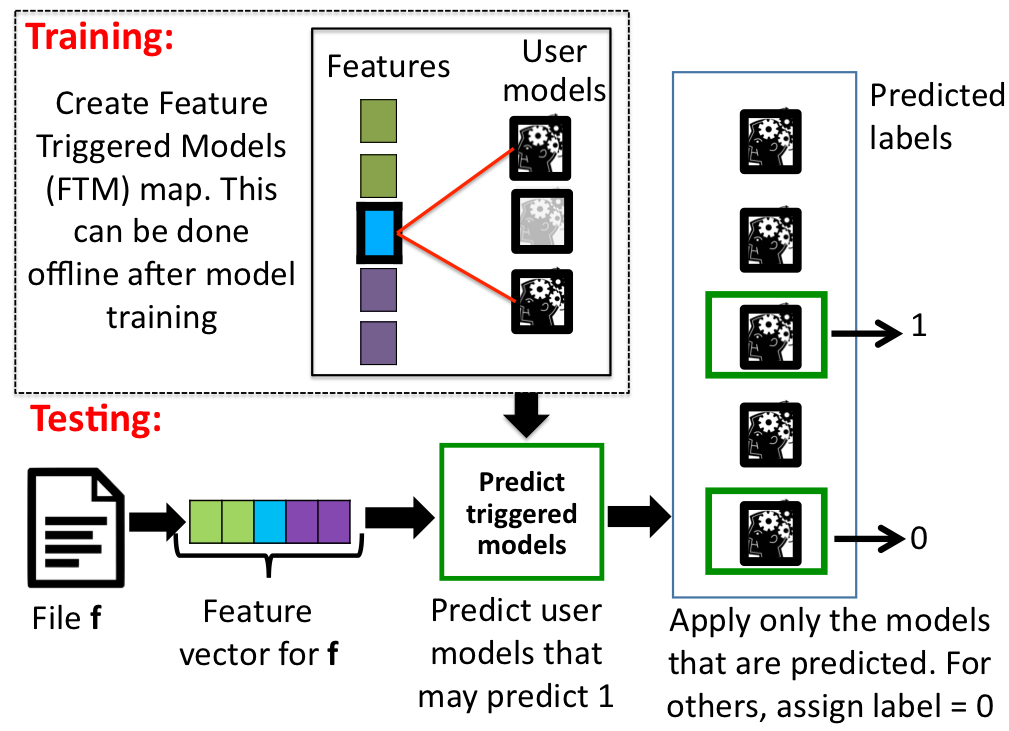
\includegraphics[width=0.75\linewidth]{FileAccess/figs/framework_withspeedup.png} 
\caption{AFMS technique first creates FTM in an offline manner.  The
  classification step applies only those models that are triggered by
  active features.}
\label{fig:speedupframework}
\end{figure}
Our technique extends the basic idea to make the optimization tunable
so that it can potentially trade-off model correctness for even better classification
efficiency.  In order to do so, we
define that {\it a feature with index $j$ triggers a model} when $w_j
\ge \tau$ or $w_0 \ge 0$ where $w_0$ and $w_j$ are the intercept and the $j^{th}$ feature weight of the model respectively. Here, we use the threshold parameter $\tau
\ge 0$ to make the technique tunable. Given a test file, a model would be applied on it 
if any of the active features of the test file \textit{trigger} the model. 
For $\tau = 0$, there is no
loss of predictive correctness, and yet there is performance gain due to the
optimization.  However, as $\tau$ increases, fewer models are
triggered, and hence there is further improvement in the performance,
albeit at the cost of predictive correctness.  With fewer models being applied,
there will be more number of 0 as the predicted labels, and hence the
recall is expected to degrade.  However, precision and likewise
F-score can degrade or improve depending on the correctness of the recommendations.
Section~\ref{sec:exptspeedup} shows that we can gain significant
efficiency at marginal cost of model correctness.  Furthermore, the technique
can be made adaptive by varying $\tau$ based on the rate of file edit
operations at a given time.

Please refer to Algorithm~\ref{algo:AFMSClassification} to understand
variable definitions, and the details of the algorithm.  As part of
pre-processing, which is done right after the training phase, for each
feature we compute the set $FTM$ (Feature Triggered Models) consisting
of models that are triggered by the feature (Figure~\ref{fig:speedupframework}).  The algorithm computes
separate sets for metadata and CF models.

The input to the classification procedure is the array $X[1 \dots
  F_{meta}]$ of metadata features corresponding to the test 
file.  The procedure produces the outputs: an array $L[1 \dots N]$
consisting of prediction label for each of the $N$ users by CF models, and an array $Y[1 \dots N]$
consisting of prediction label by metadata models.  The
procedure initializes the output arrays with $0$ values as the default labels.  It also
initializes sets $M$ and $C$ that are later used to collect triggered
metadata and CF models respectively.  The first step obtains the set
of metadata models that are triggered by the active features. The
second step applies these metadata models to compute metadata predicted labels, which are also the CF features $Y$.  The third step appends the CF features to the metadata features. 
The fourth step obtains the set of CF models that are triggered by the
active features.  Finally, the last step applies these CF models to
compute the CF predicted labels.

If a model is not applied, the default label $0$ becomes the
predicted label, and the algorithm assigns a random negative value as
the confidence score for the label.  We need the confidence score
because it is used to determine the relative ranking of test files,
which is then used in the computation of recall at 75\%.  As a side
effect, it is possible that AR@75P for AFMS with $\tau = 0$ may differ
from AR@75P computed without AFMS.


\subsubsection{Complexity analysis}  In AFMS classification procedure,
steps 2 and 5 are the most expensive ones, requiring $O(N)$
classifications.  Thus, with the rate of file edit operation
$R_{edit}$, the algorithm needs to perform $O(NR_{edit})$
classifications.  The optimization does not change the worst case time
complexity because it is possible that all the models are triggered
for a particular dataset. However, given the presence of natural
class imbalance in user-activity datasets, our optimization
significantly improves the average case time complexity.  For
instance, with $\tau = 0.5$, testing of a single file on an average
requires approximately 0.5 metadata- and 0.2 CF-based classifications out of 30
evaluation users.  This reduces the classification time of metadata
and CF models by 62 and 169 times respectively. The next section
provides detailed performance results.

%% FIXME: Why don't these numbers match the numbers in the  result
%% section 

\subsection{AFMS Evaluation}
\label{sec:exptspeedup}
%%
We measure the performance improvement using a simple metric:
%%
\begin{equation}
\label{eq:speedupgain} 
\mbox{{\it Speed-up}} = \frac{\mbox{\# models applied without AFMS}}{\mbox{\# models applied with AFMS}}.
\end{equation}
%%
Speed-up provides a direct estimate of reduction in classification
time.


\begin{figure*}
\begin{minipage}{.49\textwidth}
\centering
\epsfig{width=0.95\linewidth,figure=FileAccess/figs/gains_thresh.eps}

\captionof{figure}{Speed-up vs. $\tau$ for metadata models}
\label{fig:gainvsThreshMeta}
\end{minipage}
\begin{minipage}{.49\textwidth}
\centering
\epsfig{width=0.95\linewidth,figure=FileAccess/figs/gains_with_threshCF.eps}

\captionof{figure}{Speed-up vs. $\tau$ for CF models} 
\label{fig:gainvsThreshCF}
\end{minipage}

\end{figure*}


Figures \ref{fig:gainvsThreshMeta}-\ref{fig:r75pvsThreshCF} show the
effect of $\tau$ on speed-up, and various correctness metrics including
average precision, recall, and F-score.  The numbers are averaged across all
the evaluation users, and all training and testing periods for
individual shares.

In general, we observe that speed-up increases exponentially with
respect to $\tau$, whereas the correctness metrics degrade almost linearly,
with a mild slope, as $\tau$ increases.  This clearly shows that AFMS
can obtain significant efficiency at marginal cost of accuracy.

%%
%% FIXME: Average AF (average of average) there is no cosistency in
%% in description and graphs
%%
%% Change Y axis labels for speedup graphs (fig 10, 11): Avg speedup
%% change ``speed-up'' -> ``speedup'' consistently everywhere
%%


As expected, for $\tau = 0$, AFMS does not lose accuracy, e.g., CF
model Avg AF values from Table~\ref{tab:CollabFilteringPerf} and
Figure~\ref{fig:fscorevsThreshCF} remain the same for all shares.  And
yet, AFMS provides 4 times average speed-up across all shares for metadata models, and 
6 times average speed-up for CF models. The speed-up for $\tau = 0$ is as high as 15 times and 23 times for share A for metadata and CF models respectively. 
With $\tau = 0.5$, the average speed-up for metadata models is 62 times, and for CF models is 169 times. The most gain is observed for share A as 147 times for metadata models, and 280 times for CF models. However, this
threshold affects the correctness, dropping averages across shares. For example, for CF models, the Avg AF changed 
from 49.6\% to 45.8\%, Avg AR from 48\% to 33.3\%, Avg AR@75P from 44.8\% to 36.9\%, but
slightly improving Avg AP from 38.9\% to 42.5\%.  These results
confirm the expected effect as discussed in
Section~\ref{sec:AFMSAlgorithm}.

\comment {
Figures~\ref{fig:gainvsThreshMeta} though \ref{fig:gainvsThreshCF} show
that speed-up increases exponentially with respect to $\tau$.  In
addition, Figures~\ref{fig:precisionvsThreshMeta} through
\ref{fig:r75pvsThreshMeta} show how the precision, recall, F-score,
and Recall@75\%Precision vary with $\tau$ for metadata models on
different shares. The numbers provided are averaged across evaluation
users and across all training and testing periods.
%Figure~\ref{fig:gainvsThreshMeta} shows the variation of the speed-up averaged across all test files, evaluation users and training and testing periods. 
As expected, AFMS with $\tau=0$ leads to the same F-score as without AFMS. Despite the same predictive correctness, AFMS speeds up the testing per file by 4 times on average across all shares, and by as high as 15 times for Share A. 
%(Share A). 
For $\tau=0.5$, the average speed-up across the evaluation shares is around 62 times, and is 147 times for Share A. For the same $\tau$, average F-score drops from 47\% to 43\%, average recall drops from 47\% to 37\% and average precision drops from 35\% to 34\%. Confirming to the discussion in Section~\ref{sec:AFMSdetails}, a higher $\tau$ leads to most loss in recall. 

Figures~\ref{fig:precisionvsThreshCF} through \ref{fig:r75pvsThreshCF} show the variation of the model performance metrics with $\tau$ for CF models. 
For our experiments, we have chosen the value of $\tau$ to be the same for Metadata-FTM and CF-FTM. %Also, for the calculation of speed-up for CF models as per Eq.~\ref{eq:speedupgain}, the metadata and the CF models have been considered equivalent. 
For CF models, $\tau=0$ leads to average speed-up of more than 6 times and $\tau=0.5$ leads to average speed-up of 170 times. The speed-up observed for Share A for $\tau=0.5$ is 280 times. The observed testing speed-up demonstrates that the proposed AFMS approach can significantly reduce the testing computational requirement of the proposed file recommendation system. 
\vspace{-0.2in}
}
% Metadata models 
\begin{figure*}[htb!]
\begin{minipage}{.49\textwidth}
\centering
\epsfig{width=0.95\linewidth,figure=FileAccess/figs/precisions_thresh.eps}
%\vspace{-0.15in}
\captionof{figure}{Precision vs. $\tau$ for metadata models}
\label{fig:precisionvsThreshMeta}
\end{minipage}
\begin{minipage}{.49\textwidth}
\centering
\epsfig{width=0.95\linewidth,figure=FileAccess/figs/recalls_thresh.eps}
%\vspace{-0.15in}
\captionof{figure}{Recall vs. $\tau$ for metadata models} 
\label{fig:recallvsThreshMeta}
\end{minipage}
\begin{minipage}{.49\textwidth}
\centering
\epsfig{width=0.95\linewidth,figure=FileAccess/figs/fscore_thresh.eps}
%\vspace{-0.15in}
\captionof{figure}{F-score vs. $\tau$ for metadata models}
\label{fig:fscorevsThreshMeta}
\end{minipage}
\begin{minipage}{.49\textwidth}
\centering
\epsfig{width=0.95\linewidth,figure=FileAccess/figs/r75p_thresh.eps}
%\vspace{-0.15in}
\captionof{figure}{Recall@75\%Precision vs. $\tau$ for metadata models} 
\label{fig:r75pvsThreshMeta}
\end{minipage}
%\vspace{-0.4in}
\end{figure*}


% CF models variations with threshold: 
\begin{figure*}[htb!]
\begin{minipage}{.49\textwidth}
\centering
\epsfig{width=0.95\linewidth,figure=FileAccess/figs/precision_with_threshCF.eps}
%\vspace{-0.1in}
\captionof{figure}{Precision vs. $\tau$ for CF models}
\label{fig:precisionvsThreshCF}
\end{minipage} 
\begin{minipage}{.49\textwidth}
\centering
\epsfig{width=0.95\linewidth,figure=FileAccess/figs/recalls_with_threshCF.eps}
%\vspace{-0.1in}
\captionof{figure}{Recall vs. $\tau$ for CF models} 
\label{fig:recallvsThreshCF}
\end{minipage} 
\begin{minipage}{.49\textwidth}
\centering
\epsfig{width=0.95\linewidth,figure=FileAccess/figs/fscores_with_threshCF.eps}
%\vspace{-0.1in}
\captionof{figure}{F-score vs. $\tau$ for CF models}
\label{fig:fscorevsThreshCF}
\end{minipage} 
\begin{minipage}{.49\textwidth}
\centering
\epsfig{width=0.95\linewidth,figure=FileAccess/figs/r75p_with_threshCF.eps}
%\vspace{-0.1in}
\captionof{figure}{Recall@75\%Precision vs. $\tau$ for CF models} 
\label{fig:r75pvsThreshCF}
\end{minipage} 
\end{figure*}

\comment{
\begin{figure}
\epsfig{width=0.95\linewidth,figure=FileAccess/figs/gains_with_threshCF.eps}
\caption{Variation of average speed-up gain with $\tau$ for CF models}
\label{fig:gainvsThreshCF}
\end{figure} 
}
\comment {
\begin{figure}
\centering
\epsfig{width=0.45\linewidth,figure=FileAccess/figs/gains_vs_fscoresCF.eps}
%\vspace{-0.15in}
\caption{Variation of average speed-up gain with AF for CF models. \CV{is this figure needed?}} 
\label{fig:gainvsfscoreCF}
\end{figure}
}

\comment{
\vspace{-0.2in}
\section{Experimental validation of AFMS }
\label{sec:exptspeedup}
We measure the reduction in the testing computational requirement of a file $f$ using \textit{speed-up} defined as follows: 
\begin{equation}
\label{eq:speedupgain} 
\mbox{speed-up} = \frac{\mbox{\# models applied on $f$ without AFMS}}{\mbox{\# models applied on $f$ with AFMS}}.
\end{equation}
%\CV{speedup seemed more attention grabbing than complexity. Let me know if this fits well }
\vspace{-0.2in}
\begin{figure*}
\begin{minipage}{.49\textwidth}
\epsfig{width=\linewidth,figure=FileAccess/figs/gains_thresh.eps}
\vspace{-0.15in}
\captionof{figure}{Variation of average speed-up gain with $\tau$ for metadata models}
\label{fig:gainvsThreshMeta}
\end{minipage}
\begin{minipage}{.49\textwidth}
\epsfig{width=\linewidth,figure=FileAccess/figs/gains_with_threshCF.eps}
\vspace{-0.15in}
\captionof{figure}{Variation of average speed-up gain with $\tau$ for CF models} 
\label{fig:gainvsThreshCF}
\end{minipage}
\vspace{-0.15in}
\end{figure*}

Figures~\ref{fig:gainvsThreshMeta} and \ref{fig:gainvsThreshCF} show how the speed-up varies with $\tau$ for different shares for Metadata and CF models respectively. In addition, Figures~\ref{fig:precisionvsThreshMeta} through \ref{fig:r75pvsThreshMeta} show how the precision, recall, F-score, and Recall@75\%Precision vary with $\tau$ for metadata models on different shares. The numbers provided are averaged across evaluation users and across all training and testing periods. 
%Figure~\ref{fig:gainvsThreshMeta} shows the variation of the speed-up averaged across all test files, evaluation users and training and testing periods. 
As expected, AFMS with $\tau=0$ leads to the same F-score as without AFMS. Despite the same predictive correctness, AFMS speeds up the testing per file by 4 times on average across all shares, and by as high as 15 times for Share A. 
%(Share A). 
For $\tau=0.5$, the average speed-up across the evaluation shares is around 62 times, and is 147 times for Share A. For the same $\tau$, average F-score drops from 47\% to 43\%, average recall drops from 47\% to 37\% and average precision drops from 35\% to 34\%. Confirming to the discussion in Section~\ref{sec:AFMSdetails}, a higher $\tau$ leads to most loss in recall. 

Figures~\ref{fig:precisionvsThreshCF} through \ref{fig:r75pvsThreshCF} show the variation of the model performance metrics with $\tau$ for CF models. 
For our experiments, we have chosen the value of $\tau$ to be the same for Metadata-FTM and CF-FTM. %Also, for the calculation of speed-up for CF models as per Eq.~\ref{eq:speedupgain}, the metadata and the CF models have been considered equivalent. 
For CF models, $\tau=0$ leads to average speed-up of more than 6 times and $\tau=0.5$ leads to average speed-up of 170 times. The speed-up observed for Share A for $\tau=0.5$ is 280 times. The observed testing speed-up demonstrates that the proposed AFMS approach can significantly reduce the testing computational requirement of the proposed file recommendation system. 
\vspace{-0.2in}
% Metadata models 
\begin{figure*}[htb!]
\begin{minipage}{.49\textwidth}
\epsfig{width=0.85\linewidth,figure=FileAccess/figs/precisions_thresh.eps}
\vspace{-0.15in}
\captionof{figure}{Variation of the average precision (AP) with $\tau$ for metadata models}
\label{fig:precisionvsThreshMeta}
\end{minipage}
\begin{minipage}{.49\textwidth}
\epsfig{width=0.85\linewidth,figure=FileAccess/figs/recalls_thresh.eps}
\vspace{-0.15in}
\captionof{figure}{Variation of the average recall (AR) with $\tau$ for metadata models} 
\label{fig:recallvsThreshMeta}
\end{minipage}
\begin{minipage}{.49\textwidth}
\epsfig{width=0.85\linewidth,figure=FileAccess/figs/fscore_thresh.eps}
\vspace{-0.15in}
\captionof{figure}{Variation of the average F-score (AF) with $\tau$ for metadata models}
\label{fig:fscorevsThreshMeta}
\end{minipage}
\begin{minipage}{.49\textwidth}
\epsfig{width=0.85\linewidth,figure=FileAccess/figs/r75p_thresh.eps}
\vspace{-0.15in}
\captionof{figure}{Variation of the average recall at 75\% P (AR@75P) with $\tau$ for metadata models} 
\label{fig:r75pvsThreshMeta}
\end{minipage}
\vspace{-0.4in}
\end{figure*}

\begin{figure}[!htb]
\centering
\epsfig{width=0.45\linewidth,figure=FileAccess/figs/gains_vs_fscore.eps}
\vspace{-0.1in}
\caption{Variation of average speed-up gain with AF for metadata models \CV{is this figure needed?}} 
\label{fig:gainvsfscoreMeta}
\end{figure}

% CF models variations with threshold: 
\begin{figure*}[htb!]
\begin{minipage}{.49\textwidth}
\epsfig{width=\linewidth,figure=FileAccess/figs/precision_with_threshCF.eps}
\vspace{-0.1in}
\captionof{figure}{Variation of average precision (AP) with $\tau$ for CF models}
\label{fig:precisionvsThreshCF}
\end{minipage} 
\begin{minipage}{.49\textwidth}
\epsfig{width=\linewidth,figure=FileAccess/figs/recalls_with_threshCF.eps}
\vspace{-0.1in}
\captionof{figure}{Variation of average recall (AR) with $\tau$ for CF models} 
\label{fig:recallvsThreshCF}
\end{minipage} 
\begin{minipage}{.49\textwidth}
\epsfig{width=\linewidth,figure=FileAccess/figs/fscores_with_threshCF.eps}
\vspace{-0.1in}
\captionof{figure}{Variation of average F-score (AF) with $\tau$ for CF models}
\label{fig:fscorevsThreshCF}
\end{minipage} 
\begin{minipage}{.49\textwidth}
\epsfig{width=\linewidth,figure=FileAccess/figs/r75p_with_threshCF.eps}
\vspace{-0.1in}
\captionof{figure}{Variation of average recall at 75\% precision (AR@75P) with $\tau$ for CF models} 
\label{fig:r75pvsThreshCF}
\end{minipage} 
\end{figure*}

\begin{figure}
\centering
\epsfig{width=0.45\linewidth,figure=FileAccess/figs/gains_vs_fscoresCF.eps}
\vspace{-0.15in}
\caption{Variation of average speed-up gain with AF for CF models. \CV{is this figure needed?}} 
\label{fig:gainvsfscoreCF}
\end{figure}
}



%
%% In order to explain the proposed Active Feature based Model
%% Selection (AFMS) approach, we first provide an observation regarding linear
%% SVMs that have been used to model user access patterns in our system,
%% followed by insights learnt from actual data and trained models. We then provide details on how AFMS can be used to reduce the testing computational requirement. 

%% \textbf{Observations on linear SVM.} Given a linear SVM model $M$, the
%% predicted label for a file $f$ is calculated based on the score $M(f)$
%% where
%% \vspace{-0.1in}
%% \begin{equation} 
%% \vspace{-0.1in}
%% \label{eq:linearsvmsum}
%% M(f) = w_{0,M} + \sum_{j=1}^{N}{w_{j,M}*f_j}. 
%% \end{equation} 
%% Here, $w_{0,M} \in \mathbb{R}$ is the intercept and $w_{j,M} \in \mathbb{R}$ $\forall j \in [1,N]$ are the learnt feature weights of the trained model $M$. $f_j$ is the value of the $j^{th}$ feature of $f$ and $N$ is the number of features. The model predicts label 1 if $M(f) > 0$, and 0 otherwise. Thus if $w_{0,M}<0$, then a necessary condition for $M$ to predict 1 for file $f$ is that $f$ has at least one such feature that $M$ has positive feature weight for. Based on the above, and the fact that the defined features in Section~\ref{sec:features} are either positive or zero, the following can be concluded: The set of models that have positive feature weight for at least one of the non-zero features of a test file $f$ is a superset of the set of models that would predict label 1 for $f$. Thus given a test file $f$, it can be said that the models that do not have positive features for any of the non-zero features of $f$ would predict label 0 and need not be applied on $f$. This is the key intuition behind the proposed AFMS approach. 
%% \begin{table}
%% {\fontsize{8pt}{1em}\selectfont
%% \begin{center}
%% \begin{tabular}{|>{\centering}p{0.065\linewidth}|>{\centering}p{0.2\linewidth}|>{\centering}p{0.25\linewidth}|>{\centering}p{0.2\linewidth}|>{\centering}p{0.23\linewidth}|} \hline
%% \textbf{Share} &  \textbf{\% non-zero features} & \textbf{\% models with non-negative intercept (out of 30)} & \textbf{\% features with positive weights in models} & \textbf{\% triggered models per feature (out of 30)} \tabularnewline  \hline
%% A & 0.1 & 0.0 & 2.8 & 2.8    \tabularnewline  \hline
%% B & 1.9 & 1.1 & 2.5 & 3.6   \tabularnewline  \hline
%% C & 0.1 & 0.0 & 0.2 & 0.2  \tabularnewline  \hline
%% D & 6.6 & 0.0 & 0.8 & 0.8   \tabularnewline  \hline
%% E & 1.4 & 3.9 & 15.2 & 18.5  \tabularnewline  \hline
%% F & 1.6 & 1.7 & 4.2 & 5.8  \tabularnewline  \hline
%% G & 6.1 & 25.5 & 21.7 & 40.8  \tabularnewline  \hline
%% H & 0.01 & 0.0 & 4.1 & 4.1  \tabularnewline  \hline
%% \end{tabular}
%% \end{center}
%% }
%% \vspace{-0.1in}
%% \caption{Analysis of feature sparsity and of trained metadata based user models per share. The model statistics are averaged across 30 evaluation users and different training periods as described in Section~\ref{sec:varytraintest}. }
%% \label{tab:SpeedupPotentialStats}
%% \end{table}

%% \textbf{Insights from data and trained models.}
%% We provide below insights regarding the feature sparsity of enterprise data, and relate class bias in the trained user models with individual features. 
%% %\indent In addition to making the above observation about linear SVMs, we analyze the trained metadata user models for insights relating to the bias in the models, and the relationship between models and individual features. These are summarized below. 
%% \begin{itemize}
%% \item The features used in our system demonstrate significant sparsity. Table~\ref{tab:SpeedupPotentialStats} shows that only 0.01\% to 6.1\% of the metadata features are non zero. For CF models, it is observed that on average across all shares, only 2.1\% of the features are non zero. 
%% \item The training data for most user models has a high amount of
%%   class imbalance, favoring class 0. This is because for a typical
%%   user, most of the files observed in training period are not accessed by the user. As a result, the trained linear SVM models
%%   typically have a negative intercept (i.e., $w_{0,M} < 0$ in
%%   Eq.~\ref{eq:linearsvmsum}), suggesting the classifier has an a
%%   priori expectation of the user not accessing the file.
%% %, followed by negative or positive feature weights.
%% Table~\ref{tab:SpeedupPotentialStats} shows that for half of the eight
%% evaluation shares, all the trained metadata models have negative
%% intercepts, and that across all eight shares, only 4\% of models have
%% non-negative intercepts.
%% \item The trained models typically have positive feature weight (i.e.,
%%   $w_{j,M} > 0$ in Eq.~\ref{eq:linearsvmsum}) for only few features. Table~\ref{tab:SpeedupPotentialStats} shows that on
%%   average, the fraction of features having positive weight in trained
%%   metadata models with negative intercept is only 6.4\%.
%% \item Table~\ref{tab:SpeedupPotentialStats} also shows that each
%%   feature on average has positive weights in less than 10\% of models
%%   in a share.
%% %. On an average, the models have a positive weight for only 6.4\% of the features. 
%% %\item Among the models that have negative intercept, only XX\% of the features on an average have positive weight 
%% \end{itemize} 
%% The above insights suggest that through selecting the user models to apply on a test file, using its non zero features, it may be possible to achieve significant reduction in the testing complexity without substantial loss in model correctness. Section~\ref{sec:exptspeedup} validates our hypothesis through experiments. We provide details of the proposed approach (AFMS) below and also show how AFMS can, in addition, trade-off model correctness for further lowering of the testing complexity.
%% %This is the basis of AFMS based approach to speed-up the testing per file. 

\comment {
\subsection{AFMS Implementation}
\label{sec:AFMSdetails}
\begin{figure}[htp]
\centering
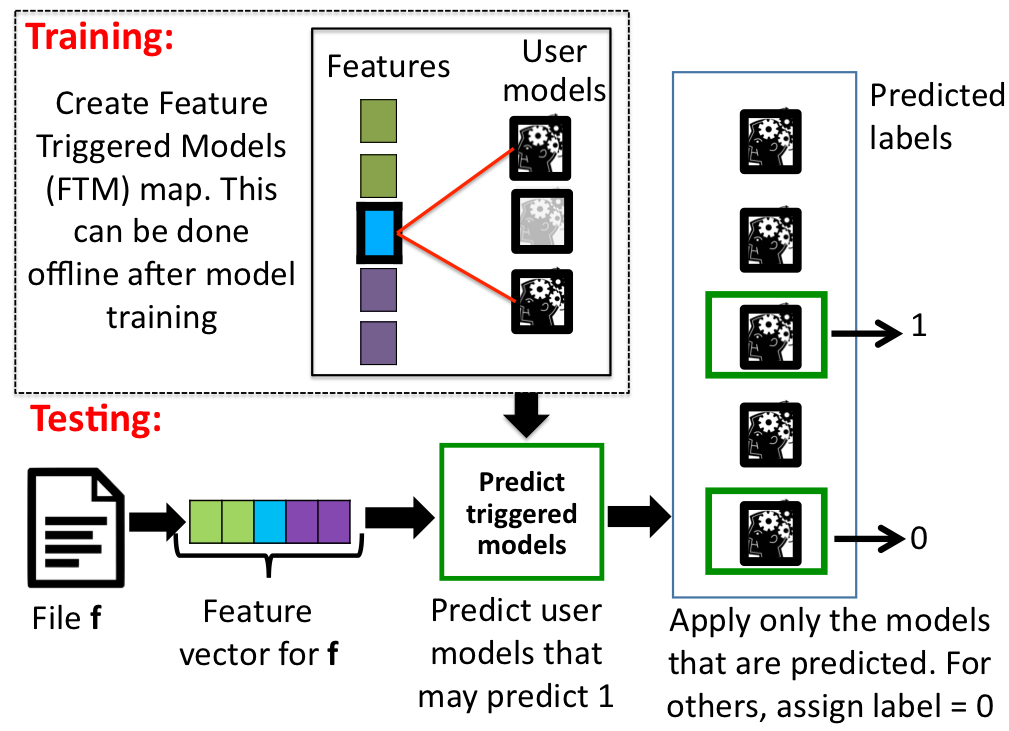
\includegraphics[width=0.7\linewidth]{FileAccess/figs/framework_withspeedup.png}
\caption{In the AFMS approach, first a Feature Triggered Models (FTM)
  map is created in an offline manner. For each test file $f$, the
  triggered models are predicted by using FTM map and only those
  models are applied on $f$. }
\label{fig:speedupframework}
\end{figure}
Figure~\ref{fig:speedupframework} shows the overall AFMS
approach. After training personalized user models, a Feature Triggered
Models (FTM) map is created to capture the user models that are \textit{triggered} by each feature. A user model $M$ is said to be \textit{triggered} by a feature $f_j$ if the feature weight for $f_j$ i.e., $w_{j,M}$ is greater than $\tau$ where $\tau \ge 0 $ is called the \textit{triggering threshold}. The value of $\tau$ determines how selective the AFMS approach is, as detailed later in this section. The FTM map needs to be
updated only when the models are re-trained. Let $N_{Meta}$ represent the number of metadata features, and let $N_{CF} = N_{Meta} + \mid\!\!U\!\!\mid$ be the number of features used in CF  models. Algorithm~\ref{alg:speedupTraining}
shows how FTM map or FTM can be obtained based on trained models. FTMs created 
using metadata models or CF models are referred to as
Metadata-FTM or CF-FTM
respectively. 

During testing of file
$f$, the \textit{triggered models} for $f$ are the set of models that
are selected to be applied on $f$ and are predicted based on the created FTM
and on the active features in $f$, i.e., the features having a non-zero for $f$. 
Algorithms~\ref{alg:speedupMetaTesting} shows how the created Metadata-FTM can be used to
obtain Triggered metadata models for test
files. For AFMS with CF models, in order to select CF models using CF-FTM, the metadata models also need to be selected using the Metadata-FTM. While using the CF-FTM, we define the active features of a file $f$ to be the non-zero metadata features of $f$ as well as the positive
predicted labels by the Triggered metadata models for $f$. This is detailed in Algorithm~\ref{alg:speedupCFTesting}. 

\begin{algorithm}[t!]
 {\fontsize{8pt}{1em}\selectfont
 \caption{Constructing FTM map}
 \label{alg:speedupTraining} 
\textbf{Input:}  
Triggering threshold: $\tau$, Trained user models (linear SVM): $M_i$ $\forall i \in [1,\mid\!\!U\!\!\mid]$ 
where $M_i$ is denoted by model parameters:  \{$w_{j,i}$\} $ \forall~j \in [0, N ]$.   \\
For Metadata-FTM, $N=N_{Meta}$ and $M_i$ represent metadata models \\ 
For CF-FTM, $N=N_{CF}$ and $M_i$ represent CF models \\ 
\textbf{Procedure: } \\
Define FTM as a hashmap mapping feature to set of models (triggered models) \\
%Initialize FTM as empty hash map\\ 
%For $i$ = 1 to $\mid\!\!U\!\!\mid$ \\ 
For each feature ($j$): \\ 
\hspace*{2mm} FTM($j$) = \{$M_i$\} s.t. $w_{j,i} \ge \tau$ \\ 
%For each user model (i.e., $M_i$) in the share \\
%\hspace*{2mm} Triggering Features = \{j : $w_{j,i} > \tau$\} \\ 
%\hspace*{2mm} For each $feat$ in Triggering Features \\ 
%\hspace*{5mm} Add user model $M_i$ as a triggered model in FTM for key = $feat$ \\ 
\textbf{Output:} FTM 
 }
 \end{algorithm}

 \begin{algorithm}[t!]
 {\fontsize{8pt}{1em}\selectfont
 \caption{Using FTM map to select metadata models} 
 \label{alg:speedupMetaTesting} 
 \textbf{Input:} 
Metadata-FTM, Test file $f$ denoted by its feature values: \{$f_j$\} $\forall j \in [1,N_{Meta}]$ \\ 
\textbf{Procedure: } 
Initialize Triggered metadata models for $f$ as empty set \\ 
Let AF($f$) := active features of $f$. AF($f$) = \{$j$\} s.t. $f_j  > 0$ \\
For each $feat$ in AF($f$): \\ 
\hspace*{2mm} Triggered metadata models for $f$ = \big\{Triggered metadata models for $f$ \\  \hspace*{45mm} $\bigcup$  Metadata-FTM($feat$) \big\} \\ 
%\hspace*{2mm} Add models in Metadata-FTM($feat$) to Triggered metadata models \\ 
\textbf{Output:} Triggered metadata models for $f$ 
 }
 \end{algorithm}

 \begin{algorithm}[t!]
 {\fontsize{8pt}{1em}\selectfont
 \caption{Using FTM map to select CF models} 
 \label{alg:speedupCFTesting} 
 \textbf{Input:} 
CF-FTM, Test file $f$  denoted by its feature values: \{$f_j$\} $\forall j \in [1,N_{CF}]$, Triggered metadata models for $f$ \\ 
\textbf{Procedure: } 
Initialize Triggered CF models for $f$ as empty set \\ 
Apply Triggered metadata models for $f$ to get predicted labels for $f$ represented by $L_{meta, f, i} \forall i \in [1, \mid\!\!U\!\!\mid] $ \\
Let AF($f$) := active features of $f$ \\ 
AF($f$) = \big\{\{$j$\} s.t. $f_j  > 0$  \, $\bigcup$  \{$N+i$\} s.t. $L_{meta, f, i} > 0 $ \big\} \\ 
For each $feat$ in AF($f$): \\ 
\hspace*{2mm} Triggered CF models for $f$ = \big\{Triggered CF models for $f$ \\  \hspace*{45mm} $\bigcup$  CF-FTM($feat$) \big\} \\ 
%\hspace*{2mm} Add models in CF-FTM($feat$) to Triggered CF models \\ 
\textbf{Output:} Triggered CF models for $f$ 
 }
 \end{algorithm}
%\vspace{-0.2in}

For $\tau=0$, the proposed AFMS approach is expected to achieve the same predictive correctness in terms of precision, recall and F-score as without AFMS, i.e., by applying every user model on each test file. When a model $M_i$ is not applied on a test file $f$, we assign its default label 0 and its confidence score to be a random negative value. 
%The test files for which a user model say $M_i$ is not applied is assigned the default label 0 and a constant value for  the confidence score. 
As a result, the ranking of the test files in terms of the prediction confidence score as per $M_i$ might be different in AFMS approach as compared to without AFMS. Since the relative ranking of test files is useful for measuring recall at 75\% precision, it is possible that AR@75P for AFMS with $\tau=0$ might differ from AR@75P without AFMS. As $\tau$ is increased, an equal or less number of models would be applied on each test file and thus the computation required per file is expected to decrease. Since less models are applied on test files, more predicted labels by the models would default to 0 and the recall is expected to degrade. By varying $\tau$, we can thus trade off the model correctness for reduction in testing computation. 
In scenarios where the available computational resources are insufficient to process the edited files, $\tau$ could be increased to process the edited files in the available resources, albeit with some loss in the predictive correctness. 
In Section~\ref{sec:exptspeedup} shows that AFMS enables a very convenient trade-off by providing significant reduction in the testing computation for marginal loss in correctness. 
Furthermore, this can also enable adaptive approaches that vary $\tau$ based on the variable rate of file edits so that more test files can be processed per unit time. 

\subsection{Complexity analysis} 
\label{sec:speedupcomplexity} 
%If for each test file, every user model in a share is applied, the average case and worst case time complexity of testing a file are both equal to $O(\mid~U~\mid)$. 
Through AFMS, the worst case testing time complexity of our system remains at $O(\mid\!\!U\!\!\mid \times R_{edit})$ since it is possible that all models in a share may be applied on the test files. However, the average case testing time complexity is $O($\textit{average number of models triggered per file}$ \times R_{edit})$. The latter may be significantly lower than the testing complexity of our system without AFMS, i.e.,  $O(\mid\!\!U\!\!\mid \times R_{edit})$. For example, it is empirically observed that for $\tau =0.5$, on average only 3.2 metadata models and 1.7 CF models are applied on test files out of 30 evaluation models. Thus on average, the testing computational requirement of our system reduces by around 9 and 18 times respectively for $\tau=0.5$. The next section provides detailed performance results for our system with AFMS. 
%Table~\ref{sec:testspeedup} shows that each feature triggers few user models and since each file has sparse features, the average number of models triggered per file can be substantially less than $\mid~U~\mid$, leading to significant testing speed-up. 
}

\comment{
\subsection{AFMS Evaluation}
\label{sec:exptspeedup}
We measure the reduction in the testing computational requirement of a file $f$ using \textit{speed-up} defined as follows: 
\begin{equation}
\label{eq:speedupgain} 
\mbox{speed-up} = \frac{\mbox{\# models applied on $f$ without AFMS}}{\mbox{\# models applied on $f$ with AFMS}}.
\end{equation}
%\CV{speedup seemed more attention grabbing than complexity. Let me know if this fits well }
\vspace{-0.2in}
\begin{figure*}
\begin{minipage}{.49\textwidth}
\epsfig{width=\linewidth,figure=FileAccess/figs/gains_thresh.eps}
\vspace{-0.15in}
\captionof{figure}{Variation of average speed-up gain with $\tau$ for metadata models}
\label{fig:gainvsThreshMeta}
\end{minipage}
\begin{minipage}{.49\textwidth}
\epsfig{width=\linewidth,figure=FileAccess/figs/gains_with_threshCF.eps}
\vspace{-0.15in}
\captionof{figure}{Variation of average speed-up gain with $\tau$ for CF models} 
\label{fig:gainvsThreshCF}
\end{minipage}
\vspace{-0.15in}
\end{figure*}

Figures~\ref{fig:gainvsThreshMeta} and \ref{fig:gainvsThreshCF} show how the speed-up varies with $\tau$ for different shares for Metadata and CF models respectively. In addition, Figures~\ref{fig:precisionvsThreshMeta} through \ref{fig:r75pvsThreshMeta} show how the precision, recall, F-score, and Recall@75\%Precision vary with $\tau$ for metadata models on different shares. The numbers provided are averaged across evaluation users and across all training and testing periods. 
%Figure~\ref{fig:gainvsThreshMeta} shows the variation of the Speed-up averaged across all test files, evaluation users and training and testing periods. 
As expected, AFMS with $\tau=0$ leads to the same F-score as without AFMS. Despite the same predictive correctness, AFMS speeds up the testing per file by 4 times on average across all shares, and by as high as 15 times for Share A. 
%(Share A). 
For $\tau=0.5$, the average speed-up across the evaluation shares is around 62 times, and is 147 times for Share A. For the same $\tau$, average F-score drops from 47\% to 43\%, average recall drops from 47\% to 37\% and average precision drops from 35\% to 34\%. Confirming to the discussion in Section~\ref{sec:AFMSdetails}, a higher $\tau$ leads to most loss in recall. 

Figures~\ref{fig:precisionvsThreshCF} through \ref{fig:r75pvsThreshCF} show the variation of the model performance metrics with $\tau$ for CF models. 
For our experiments, we have chosen the value of $\tau$ to be the same for Metadata-FTM and CF-FTM. %Also, for the calculation of speed-up for CF models as per Eq.~\ref{eq:speedupgain}, the metadata and the CF models have been considered equivalent. 
For CF models, $\tau=0$ leads to average speed-up of more than 6 times and $\tau=0.5$ leads to average speed-up of 170 times. The speed-up observed for Share A for $\tau=0.5$ is 280 times. The observed testing speed-up demonstrates that the proposed AFMS approach can significantly reduce the testing computational requirement of the proposed file recommendation system. 
\vspace{-0.2in}
% Metadata models 
\begin{figure*}[htb!]
\begin{minipage}{.49\textwidth}
\epsfig{width=\linewidth,figure=FileAccess/figs/precisions_thresh.eps}
\vspace{-0.15in}
\captionof{figure}{Variation of the average precision (AP) with $\tau$ for metadata models}
\label{fig:precisionvsThreshMeta}
\end{minipage}
\begin{minipage}{.49\textwidth}
\epsfig{width=\linewidth,figure=FileAccess/figs/recalls_thresh.eps}
\vspace{-0.15in}
\captionof{figure}{Variation of the average recall (AR) with $\tau$ for metadata models} 
\label{fig:recallvsThreshMeta}
\end{minipage}
\begin{minipage}{.49\textwidth}
\epsfig{width=\linewidth,figure=FileAccess/figs/fscore_thresh.eps}
\vspace{-0.15in}
\captionof{figure}{Variation of the average F-score (AF) with $\tau$ for metadata models}
\label{fig:fscorevsThreshMeta}
\end{minipage}
\begin{minipage}{.49\textwidth}
\epsfig{width=\linewidth,figure=FileAccess/figs/r75p_thresh.eps}
\vspace{-0.15in}
\captionof{figure}{Variation of the average recall at 75\% P (AR@75P) with $\tau$ for metadata models} 
\label{fig:r75pvsThreshMeta}
\end{minipage}
\vspace{-0.4in}
\end{figure*}

\comment{
\begin{figure}[!htb]
\epsfig{width=0.45\linewidth,figure=FileAccess/figs/gains_thresh.eps}
\vspace{-0.1in}
\caption{Variation of average speed-up gain with $\tau$ for metadata models}
\label{fig:gainvsThreshMeta}
\vspace{-0.15in}
\end{figure}
}
\begin{figure}[!htb]
\centering
\epsfig{width=0.45\linewidth,figure=FileAccess/figs/gains_vs_fscore.eps}
\vspace{-0.1in}
\caption{Variation of average speed-up gain with AF for metadata models \CV{is this figure needed?}} 
\label{fig:gainvsfscoreMeta}
\end{figure}

% CF models variations with threshold: 
\begin{figure*}[htb!]
\begin{minipage}{.49\textwidth}
\epsfig{width=\linewidth,figure=FileAccess/figs/precision_with_threshCF.eps}
\vspace{-0.1in}
\captionof{figure}{Variation of average precision (AP) with $\tau$ for CF models}
\label{fig:precisionvsThreshCF}
\end{minipage} 
\begin{minipage}{.49\textwidth}
\epsfig{width=\linewidth,figure=FileAccess/figs/recalls_with_threshCF.eps}
\vspace{-0.1in}
\captionof{figure}{Variation of average recall (AR) with $\tau$ for CF models} 
\label{fig:recallvsThreshCF}
\end{minipage} 
\begin{minipage}{.49\textwidth}
\epsfig{width=\linewidth,figure=FileAccess/figs/fscores_with_threshCF.eps}
\vspace{-0.1in}
\captionof{figure}{Variation of average F-score (AF) with $\tau$ for CF models}
\label{fig:fscorevsThreshCF}
\end{minipage} 
\begin{minipage}{.49\textwidth}
\epsfig{width=\linewidth,figure=FileAccess/figs/r75p_with_threshCF.eps}
\vspace{-0.1in}
\captionof{figure}{Variation of average recall at 75\% precision (AR@75P) with $\tau$ for CF models} 
\label{fig:r75pvsThreshCF}
\end{minipage} 
\end{figure*}

\comment{
\begin{figure}
\epsfig{width=0.95\linewidth,figure=FileAccess/figs/gains_with_threshCF.eps}
\caption{Variation of average speed-up gain with $\tau$ for CF models}
\label{fig:gainvsThreshCF}
\end{figure} 
}
\begin{figure}
\centering
\epsfig{width=0.45\linewidth,figure=FileAccess/figs/gains_vs_fscoresCF.eps}
\vspace{-0.15in}
\caption{Variation of average speed-up gain with AF for CF models. \CV{is this figure needed?}} 
\label{fig:gainvsfscoreCF}
\end{figure}


\comment{
\vspace{-0.2in}
\section{Experimental validation of AFMS }
\label{sec:exptspeedup}
We measure the reduction in the testing computational requirement of a file $f$ using \textit{speed-up} defined as follows: 
\begin{equation}
\label{eq:speedupgain} 
\mbox{speed-up} = \frac{\mbox{\# models applied on $f$ without AFMS}}{\mbox{\# models applied on $f$ with AFMS}}.
\end{equation}
%\CV{speedup seemed more attention grabbing than complexity. Let me know if this fits well }
\vspace{-0.2in}
\begin{figure*}
\begin{minipage}{.49\textwidth}
\epsfig{width=\linewidth,figure=FileAccess/figs/gains_thresh.eps}
\vspace{-0.15in}
\captionof{figure}{Variation of average speed-up gain with $\tau$ for metadata models}
\label{fig:gainvsThreshMeta}
\end{minipage}
\begin{minipage}{.49\textwidth}
\epsfig{width=\linewidth,figure=FileAccess/figs/gains_with_threshCF.eps}
\vspace{-0.15in}
\captionof{figure}{Variation of average speed-up gain with $\tau$ for CF models} 
\label{fig:gainvsThreshCF}
\end{minipage}
\vspace{-0.15in}
\end{figure*}

Figures~\ref{fig:gainvsThreshMeta} and \ref{fig:gainvsThreshCF} show how the speed-up varies with $\tau$ for different shares for Metadata and CF models respectively. In addition, Figures~\ref{fig:precisionvsThreshMeta} through \ref{fig:r75pvsThreshMeta} show how the precision, recall, F-score, and Recall@75\%Precision vary with $\tau$ for metadata models on different shares. The numbers provided are averaged across evaluation users and across all training and testing periods. 
%Figure~\ref{fig:gainvsThreshMeta} shows the variation of the speed-up averaged across all test files, evaluation users and training and testing periods. 
As expected, AFMS with $\tau=0$ leads to the same F-score as without AFMS. Despite the same predictive correctness, AFMS speeds up the testing per file by 4 times on average across all shares, and by as high as 15 times for Share A. 
%(Share A). 
For $\tau=0.5$, the average speed-up across the evaluation shares is around 62 times, and is 147 times for Share A. For the same $\tau$, average F-score drops from 47\% to 43\%, average recall drops from 47\% to 37\% and average precision drops from 35\% to 34\%. Confirming to the discussion in Section~\ref{sec:AFMSdetails}, a higher $\tau$ leads to most loss in recall. 

Figures~\ref{fig:precisionvsThreshCF} through \ref{fig:r75pvsThreshCF} show the variation of the model performance metrics with $\tau$ for CF models. 
For our experiments, we have chosen the value of $\tau$ to be the same for Metadata-FTM and CF-FTM. %Also, for the calculation of speed-up for CF models as per Eq.~\ref{eq:speedupgain}, the metadata and the CF models have been considered equivalent. 
For CF models, $\tau=0$ leads to average speed-up of more than 6 times and $\tau=0.5$ leads to average speed-up of 170 times. The speed-up observed for Share A for $\tau=0.5$ is 280 times. The observed testing speed-up demonstrates that the proposed AFMS approach can significantly reduce the testing computational requirement of the proposed file recommendation system. 
\vspace{-0.2in}
% Metadata models 
\begin{figure*}[htb!]
\begin{minipage}{.49\textwidth}
\epsfig{width=\linewidth,figure=FileAccess/figs/precisions_thresh.eps}
\vspace{-0.15in}
\captionof{figure}{Variation of the average precision (AP) with $\tau$ for metadata models}
\label{fig:precisionvsThreshMeta}
\end{minipage}
\begin{minipage}{.49\textwidth}
\epsfig{width=\linewidth,figure=FileAccess/figs/recalls_thresh.eps}
\vspace{-0.15in}
\captionof{figure}{Variation of the average recall (AR) with $\tau$ for metadata models} 
\label{fig:recallvsThreshMeta}
\end{minipage}
\begin{minipage}{.49\textwidth}
\epsfig{width=\linewidth,figure=FileAccess/figs/fscore_thresh.eps}
\vspace{-0.15in}
\captionof{figure}{Variation of the average F-score (AF) with $\tau$ for metadata models}
\label{fig:fscorevsThreshMeta}
\end{minipage}
\begin{minipage}{.49\textwidth}
\epsfig{width=\linewidth,figure=FileAccess/figs/r75p_thresh.eps}
\vspace{-0.15in}
\captionof{figure}{Variation of the average recall at 75\% P (AR@75P) with $\tau$ for metadata models} 
\label{fig:r75pvsThreshMeta}
\end{minipage}
\vspace{-0.4in}
\end{figure*}

\comment{
\begin{figure}[!htb]
\epsfig{width=0.45\linewidth,figure=FileAccess/figs/gains_thresh.eps}
\vspace{-0.1in}
\caption{Variation of average speed-up gain with $\tau$ for metadata models}
\label{fig:gainvsThreshMeta}
\vspace{-0.15in}
\end{figure}
}
\begin{figure}[!htb]
\centering
\epsfig{width=0.45\linewidth,figure=FileAccess/figs/gains_vs_fscore.eps}
\vspace{-0.1in}
\caption{Variation of average speed-up gain with AF for metadata models \CV{is this figure needed?}} 
\label{fig:gainvsfscoreMeta}
\end{figure}

% CF models variations with threshold: 
\begin{figure*}[htb!]
\begin{minipage}{.49\textwidth}
\epsfig{width=\linewidth,figure=FileAccess/figs/precision_with_threshCF.eps}
\vspace{-0.1in}
\captionof{figure}{Variation of average precision (AP) with $\tau$ for CF models}
\label{fig:precisionvsThreshCF}
\end{minipage} 
\begin{minipage}{.49\textwidth}
\epsfig{width=\linewidth,figure=FileAccess/figs/recalls_with_threshCF.eps}
\vspace{-0.1in}
\captionof{figure}{Variation of average recall (AR) with $\tau$ for CF models} 
\label{fig:recallvsThreshCF}
\end{minipage} 
\begin{minipage}{.49\textwidth}
\epsfig{width=\linewidth,figure=FileAccess/figs/fscores_with_threshCF.eps}
\vspace{-0.1in}
\captionof{figure}{Variation of average F-score (AF) with $\tau$ for CF models}
\label{fig:fscorevsThreshCF}
\end{minipage} 
\begin{minipage}{.49\textwidth}
\epsfig{width=\linewidth,figure=FileAccess/figs/r75p_with_threshCF.eps}
\vspace{-0.1in}
\captionof{figure}{Variation of average recall at 75\% precision (AR@75P) with $\tau$ for CF models} 
\label{fig:r75pvsThreshCF}
\end{minipage} 
\end{figure*}

\comment{
\begin{figure}
\epsfig{width=0.95\linewidth,figure=FileAccess/figs/gains_with_threshCF.eps}
\caption{Variation of average speed-up gain with $\tau$ for CF models}
\label{fig:gainvsThreshCF}
\end{figure} 
}
\begin{figure}
\centering
\epsfig{width=0.45\linewidth,figure=FileAccess/figs/gains_vs_fscoresCF.eps}
\vspace{-0.15in}
\caption{Variation of average speed-up gain with AF for CF models. \CV{is this figure needed?}} 
\label{fig:gainvsfscoreCF}
\end{figure}
}
}
